%
%	Praxisbezug
%

\pagebreak
\section{mTLS Analysis}

\onehalfspacing

\subsection{Resource Consumption}

To evaluate the two service meshes, we will look at the following Kubernetes metrics:\footnote{See \textit{Kubernetes (2023)}: Resource Pipeline. \cite{resPipeline}}

\begin{itemize}
    \item Number of pods
    \item CPU reserved
    \item CPU used
    \item Memory reserved
    \item Memory used
\end{itemize}

We will take the values from the Rancher cluster dashboard for each experiment iteration.

\begin{figure}[H]
\centering
\caption {Cluster Dashboard}
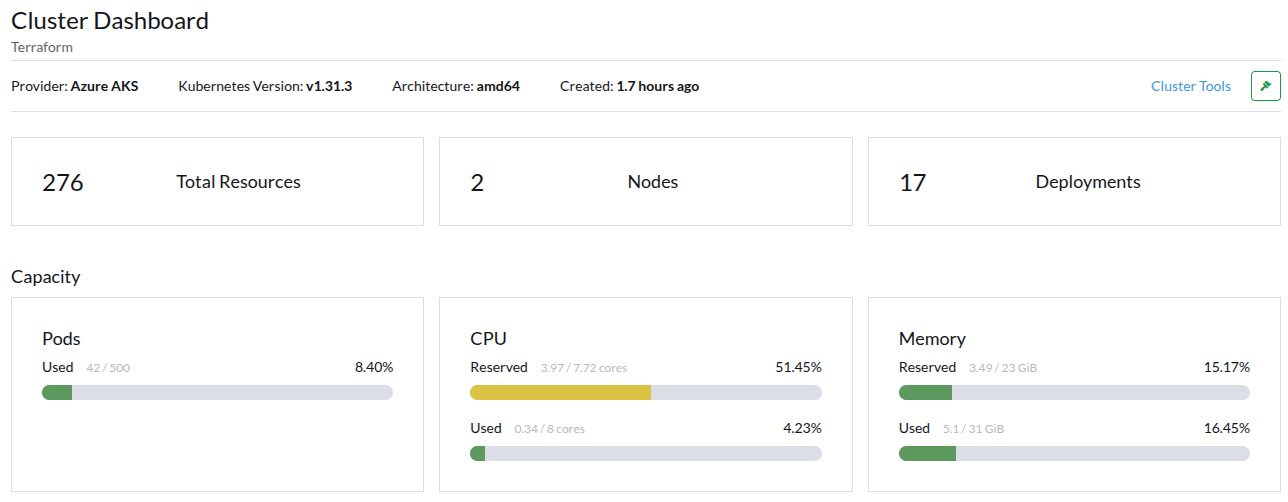
\includegraphics[width=\linewidth]{images/cluster-dashboard.png}
\label{fig:clusterDashboard}
\end{figure}

Here are the tabulated results from the experiment:

\begin{table}[ht]
  \caption{Resource Consumption}
    \begin{tabular}{| l | l | l | l | l | l |}
    \hline
    & Pods & CPU Rsvd & CPU Used & Memory Rsvd & Memory Used \\
    \hline\hline
    Idle & 37 & 3.97 cores & 0.32 cores & 3.49 GB & 4.78 GB \\
    \hline
    App Only & 42 & 3.97 cores & 0.34 cores & 3.49 GB & 5.1 GB \\
    \hline
    Linkerd & 59 & 3.97 cores & 0.61 cores & 3.49 GB & 13 GB \\
    \hline
    Istio & 61 & 5.93 cores & 1.02 cores & 7.14 GB & 13 GB \\
    \hline
    \hline
    \end{tabular}
  \label{tab:resUsage}
\end{table}

\subsection{Installation Time}

Installing the two service meshes was not very time-consuming. We measured the time from the beginning of the first command until after the Helm chart was finished installing the software.

\begin{table}[ht]
  \caption{Installation Time}
    \begin{tabular}{| l | l |}
    \hline
    & Time \\
    \hline\hline
    Linkerd & 5 min \\
    \hline
    Istio & 20 min \\
    \hline
    \hline
    \end{tabular}
  \label{tab:installTime}
\end{table}

Istio requires several prerequisites, such as a running monitoring stack, which makes the installation significantly longer.

The documentation made enabling mTLS for our sample application straightforward, either from the CLI or through auto-injection. We measured the time it took to enable mTLS on the installed sample application.

\begin{table}[ht]
  \caption{Enabling mTLS}
    \begin{tabular}{| l | l |}
    \hline
    & Time \\
    \hline\hline
    Linkerd & 5 min \\
    \hline
    Istio & 5 min \\
    \hline
    \hline
    \end{tabular}
  \label{tab:enableTime}
\end{table}

There was no difference in time or effort between Istio and Linkerd regarding enabling mTLS for our sample application.

\subsection{Findings from Linkerd}

\subsection{Findings from Istio}

\subsection{Linkerd and Istio Evaluation}

\subsection{Outlook}
